\documentclass{standalone}
\usepackage{tikz}
\usepackage{amsmath}
\usetikzlibrary{positioning}

\tikzset{main node/.style={circle,,draw,minimum size=1cm,inner sep=0pt} }
\begin{document}

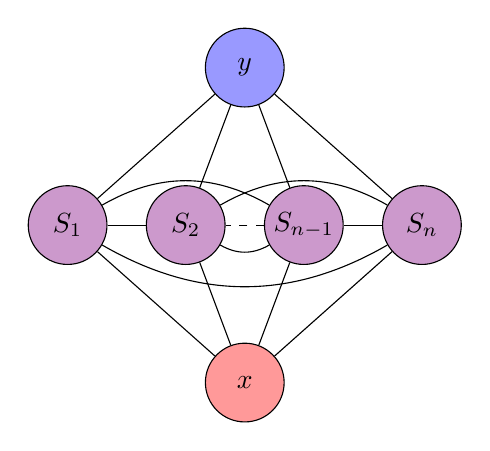
\begin{tikzpicture}
\begin{scope}[on grid]

  
  \node[main node,fill=violet!40] (1) {$S_1$};
  \node[main node, fill=violet!40] (2) [right =1.5cm of 1] {$S_2$};
  \node[main node, fill=violet!40] (3) [right =1.5cm of 2] {$S_{n-1}$};
  \node[main node, fill=violet!40] (4) [right =1.5cm of 3] {$S_n$};
  
 \node[main node, fill=red!40] (5) [below right = 2cm and 0.75cm of 2]{$x$};
 \node[main node, fill=blue!40] (6) [above right = 2cm and 0.75of 2]{$y$};
 
    \path[every node/.style={font=\sffamily\small}]
    (2) edge [-] (1)
    (3) edge [-, dashed] (2)
    (4) edge [-] (3)
    
    (5) edge [-] (1)
    (5) edge [-] (2)
    (5) edge [-] (3)
    (5) edge [-] (4)
    
    (6) edge [-] (1)
    (6) edge [-] (2)
    (6) edge [-] (3)
    (6) edge [-] (4)
    
    (3) edge [-, bend right] (1)
    (4) edge [-, bend left] (1)
    (3) edge [- ,bend left] (2)
    (4) edge [- ,bend right] (2)
    ;
    \end{scope}
\end{tikzpicture}
\end{document}